\documentclass{book}

\usepackage{bm}
\usepackage{float}
\usepackage{amsmath}
\usepackage{amsfonts}
\usepackage{graphicx}
\usepackage{lineno}
\usepackage{natbib}
\usepackage[pdftex]{hyperref}
\usepackage{soul}
\usepackage{color}
\usepackage{ctable}
\usepackage{verbatim}

\bibliographystyle{asa}

\floatstyle{plain}
\floatname{panel}{Panel}
\newfloat{algorithm}{h}{txt}[chapter]
\newfloat{panel}{h}{txt}[chapter]

\linenumbers

\begin{document}




\chapter{
Spatial Mark-Resight Models
}

\markboth{Spatial mark-resight models}{}
\label{chapt.partialID}

\vspace{.3in}


Throughout most of this book we have dealt with the situation where
all individuals are identifiable upon encounter because they
carry some form of individual mark. In Chapt. \ref{chapt.scr-unmarked}
we introduced and developed an SCR model for non-identifiable
populations, a spatial {\it non}-capture-recapture model, if you will.
These two extremes are common in the study of animal populations with
non-invasive sampling methods. However, there is also an intermediate
situation where part of the population is tagged or otherwise marked
and can thus be identified upon recapture, while the unmarked portion
remains unidentifiable.  In this situation so-called mark-resight
models \citep{bartmann_etal:1987, arnason_etal:1991, neal_etal:1993}
can be used to estimate population size and density by combining data
from both the marked and unmarked individuals.

Traditionally, capture-recapture studies involved physical capture and
marking of individuals throughout the study.  This methodology is
still widely applied in the study of species that are relatively easy
to capture, such as small mammals, but can be very costly,
logistically challenging and risky when dealing with larger
species. In contrast, in mark-resight studies a sample of individuals
is captured and tagged (or otherwise marked) during a single marking
event. Marking is followed by resighting surveys, upon which both the
detection of marked 
and unmarked animals
is recorded. Resighting surveys are usually non-invasive (hence the
name `resighting'), so that they don't involve handling of animals. As
such, mark-resight models have a major advantage over traditional
capture-recapture models in that they only require individuals to be
captured and handled once, during the initial marking. This reduces
field costs and risks for the animals (and potentially the
researchers).

Mark-resight models have a set of underlying assumptions, most of
which are identical to those of capture-recapture models; e.g.,
demographic population closure (violation of geographic population
closure can be accommodated by some models) and no loss or
misidentification of marks (see also Chapt.~\ref{chapt.scr0}).  Just
like standard capture-recapture models, there are means to incorporate
heterogeneity in capture probability. An essential assumption of
mark-resight models is that the marked individuals are a
representative sample of the study population, so that inference about
detection can be made for the whole population from the marked
sample. While this is also an implicit assumption of capture-recapture
models, in mark-resight models this means that the process of marking
individuals requires careful consideration in order to produce a
random sample.  This assumption is usually addressed by employing a
different method for marking than for resighting.


Owing to the advantages of mark-resight over capture-recapture,
especially when dealing with hard-to-trap species, mark-resight is a
popular tool in wildlife population studies. The method has been
applied for decades
to a suite of species and survey techniques,
ranging from banding and resighting Canada geese
\citep{hestbeck_malecki:1989} to ear-tagging and camera-trapping
grizzly bears \citep{mace_etal:1994} to paintball marking and areal
resightings of large ungulates \citep{skalski_etal:2005jwm}.

In this chapter we consider mark-resight within
a spatial context and
develop a spatial mark-resight (SMR) model. To motivate this model
development, imagine you conduct a live-trapping study during which
you capture and mark a number of animals with individually
recognizable tags. Subsequently, you go back out to the field and
conduct resighting surveys on an array of locations, and during these
resighting surveys you see some of your marked individuals as well as
new, unmarked ones. Then, for the marked animals you obtain the same
type of spatially explicit individual encounter histories as you would
in a standard SCR study. In addition, you obtain site (and occasion)
specific counts of individuals you did not tag. Thus, spatial
mark-resight is an SCR framework for populations where only a portion of
the individuals can be identified. The major difference between SCR
and SMR is how we include those counts of unmarked individuals in the
model. 

In the following sections we first provide some background
information on mark-resight and the types of data such surveys can
provide. We will further explore the implications of the assumption of
the marked individuals being a random subset of the population, which,
in the context of SMR models refers to both the \emph{demographic
  composition}, but also to the \emph{spatial distribution} of the
marked individuals in ${\cal S}$. 
In many real life sampling situations, this assumption will not hold
-- animals will most often be marked in some region that does not
represent the entire state-space. As a result, the distribution of marked individuals will \emph{not} follow a homogeneous point process, but their activity centers will be concentrated in the vicinity of where marking took place. 
For the sake of model development, however, throughout the central part of this chapter we will make the assumption that marked animals are a random sample from the population in ${\cal S}$. We will show that SMR models are hybrids of regular SCR models and the models
presented in Chapt. \ref{chapt.scr-unmarked} for data where
individuals cannot be uniquely identified. We explore models for both
known and unknown numbers of marked individuals, and for imperfect
individual identification of marks, and approaches to incorporate
telemetry location data. In the spatial framework, most of the
information on model parameters comes from the marked individuals. But
in Sec. \ref{partialID.sec.info} we will see that, analogous to the
models we developed previously in Chapt. \ref{chapt.scr-unmarked}, the
spatial correlation in counts of unmarked individuals also contributes
information about detection and movement. 
We conclude the chapter by presenting some general strategies of addressing a situation where marked individuals are not a random sample from ${\cal S}$. 


\section{Background}

Before we start exploring spatial mark-resight approaches in more
detail, we need to establish some terminology and gain a clear
understanding of what types of mark-resight data we can have, in order
to appreciate and understand the different flavors of mark-resight
models.

\subsection{Resighting techniques}
As with capture-recapture surveys, there are numerous methods suitable
for obtaining resightings. Common methods are visits to a set of points
for resightings by an observer, or camera-trapping; but resightings
need not be restricted to a particular set of locations. We can just
as well envision a search-encounter kind of method, where a certain
area is searched, systematically or opportunistically, for marked
animals (see Chapt. \ref{chapt.search-encounter}). In this chapter we
will only deal with fixed location resighting surveys, and we will
refer to the set of resighting locations as the resighting array. In
some instances we will also be concerned with where marked animals
were captured, and we refer to these locations as the marking
locations.

\subsection{Types of mark-resighting data}

In general, we have (at least) two sets of data: encounter histories
for marked, and thus, identifiable individuals $i$ at resighting
location $j$ and occasion $k$, $y_{ijk}$, and counts of unmarked
records, $n_{jk}$, for each resighting location $j$ and occasion $k$.
Depending on the sampling technique, we can conceive of three slightly
different types of partial ID data.


{\flushleft \bf (1) Known number of marked individuals:} If you
implement a resighting survey shortly after the marking session, you
may be confident that none of the marked individuals have died or lost
their mark. Under these circumstances you know that the number of
marked individuals available for resighting, $m$, is equal to the
number of individuals you marked. Alternatively, the marking technique
might involve radio-transmitters, allowing you to confirm the presence
or absence of marked individuals in the resighting survey area using
radio-telemetry \citep{white_shenk:2001}. In both cases, you know the
number of marked individuals in the surveyed population.  In this
situation, even though you may fail to resight some of the marked
individuals, you know how many there are, and so you can simply assign
all-zero encounter histories to the marked individuals not encountered
-- in other words, contrary to regular capture-recapture models, in
mark-resight models with a known number of marked individuals, we can
observe all-zero encounter histories. Under these circumstances,
estimating $N$ reduces to estimating the number of unmarked
individuals, $U$.

{\flushleft \bf (2) Unknown number of marked individuals:} If $m$ is
not known, for example because we suspect that some of the marks may
have been lost between tagging and conducting the resighting surveys,
we obtain a slightly different type of mark-resight data. Here, we do
not accurately know the number of marked individuals available for
resighting. As a consequence, individuals have to be resighted at
least once for us to know they are still marked and alive and thus
available for resighting. So, contrary to the situation where we know
$m$ and analogous to regular capture-recapture models, we cannot
observe all-zero encounter histories of marked individual. In this
situation, estimating $N$ involves estimating both $m$ and $U$.

A special case of this kind of data can arise from camera
trapping. Even when dealing with a species that has no spots or
stripes, some individuals in the study population can have natural
marks that make them identifiable on pictures, such as scars or a
distinct coloration. In this scenario an individual has to be
photographed at least once to be known. Here, the fact that both the
``marking'' method and the subsequent resighting method are the same
(although marking in this case does not involve any actual physical
marking) can be cause for concern: our sample of ``marked''
individuals may not be a random sample of the population but consist
of individuals that for some reason are more likely to be
photographed (e.g., individuals with activity center more interior to
the trap array). In that case, a basic assumption of the mark-resight
model is violated.

{\flushleft \bf (3) Unknown marked status:} Finally, consider a scat
or hair snare survey, where only a part of the sample is analyzed
genetically (or DNA can only be extracted from a subset of samples due
to sample quality). In this scenario, $n_{jk}$ can contain both
completely unknown individuals that are not represented at all in the
complete set of encounter histories of marked animals, {\bf $Y$}, but
it can also contain samples from individuals that we previously
identified. The difference is that in the first two scenarios, part of
the population of individuals is identifiable, while in the third
scenario, part of the sample of individuals is identifiable. This type
of data violates one of the basic assumptions of mark-resight models,
namely, that marked individuals are always correctly identified as
such.

To our knowledge there are currently no mark-resight models available
that account for possible misidentification of the marking status of
individuals (although some literature is available on
misidentification of individuals in capture-recapture studies, e.g.,
\citealp{yoshizaki_etal:2009, lukacs_burnham:2005,
  link_etal:2010}). In this chapter we will ignore this kind of data
and focus instead on types (1) and (2).

For both types of data a slightly different situation arises when
we can only tell that an individual is marked, but not
who it is. You may be able to see that an individual is marked but the
identifying feature of the tag (a number or coloration) may have
become unreadable, or may be hidden from view. In this case, in
addition to the observed $y_{ijk}$ and $n_{jk}$, you also observe a number of
sightings of marked but unidentified individuals, say $r_{jk}$.

\subsection{A short history of mark-resight models}

Initially, mark-resight methods focused on radio-tagged individuals to
estimate population size \citep{white_shenk:2001}. Radio-collars
provide a means of determining which of the animals are in the study
area and available for sampling, thus determining the number of marked
individuals in the population. Knowing this number was a prerequisite
for most earlier mark-resight approaches \citep{white:1996}. The
oldest mark-resight model is the good old Lincoln-Petersen estimator,
where individuals are marked and a single resight/recapture occasion
is carried out \citep{krebs:1999}. We need not identify individuals,
but only to tell apart marked from unmarked individuals. Let $m$ be
the number of marked individuals in the population, $m_{(R)}$ the
number of marked individuals seen on the resighting occasion, and
$n_{(R)}$ the total number of marked and unmarked individuals observed
during resighting. Population size $N$ is then estimated as
\[
N = m \times n_{(R)}/m_{(R)}.
\]

Mark-resight models using individual capture histories
over several resighting occasions were developed in the 1980s and
90s and compiled into the program \textbf{NOREMARK} \citep{white:1996}. Apart
from the basic model with known number of marked individuals and no
individual variation in resighting probabilities (joint hypergeometric
maximum likelihood estimator) \citep{bartmann_etal:1987,
  white_garrot:1990, neal:1990, neal_etal:1993}, \textbf{NOREMARK} contains
models that account for lack of geographic population closure
\citep{neal_etal:1993}, individual heterogeneity in resighting rates
and sampling with replacement (i.e. individuals can be seen more than
once on any occasion, \citep{minta_mangel:1989, bowden:1993}). A first
mark-resight model allowing for an unknown number of marked
individuals was developed by \citet{arnason_etal:1991}.

While many of these models perform well under certain situations, they
are somewhat limited in that they do not allow for combining data
across several surveys \citep{mcclintock_etal:2006} and not all of
them are likelihood-based or allow for different parameterizations
(e.g., including a time effect on detection), so that selection of the
most appropriate model cannot be based on standard approaches such as
AIC, but is largely left up to educated guesswork
\citep{mcclintock_etal:2006}. Recently, more flexible and generalized
likelihood-based mark-resight models have been developed. These models
can account for individual heterogeneity in detection, unknown number
of marked individuals and lack of geographical closure, as well as a
less than 100\% individual identification rate of marked individuals;
they can be applied to sampling with and without replacement and can
combine data across several primary sampling occasions in a robust
design type of analysis
\citep{mcclintock_etal:2009biometrics,mcclintock_etal:2009mdp}. Since
they are all likelihood-based, model selection among different
parameterizations and model averaging based on AIC is an option. Most
of these models have also been incorporated into the program {\bf
  MARK} \citep{mcclintock_white:2010}.

For a detailed treatment of these different non-spatial mark-resight
models, we refer you to the original papers cited in the preceding
paragraph. In short, these models are based on the joint likelihood of
two model components: one describing the resighting process of marked
individuals and one describing the number of unmarked individuals
observed.  The resighting process of marked individuals can use either
a Poisson or a Bernoulli observation model, depending on whether
sampling is with or without replacement, and the resighting
probabilities can have both fixed effects to model individual and
environmental covariates, and a random-effect component to accommodate
variation in detection due to individual heterogeneity.  The process
describing the number of unmarked individuals observed (or, under a
Poisson observation model, the number of times unmarked individuals
are observed), $n_t$ ($t$ here and in the following description
denotes a primary sampling occasion, for example, a year or a season)
which are approximated as a normal distribution
\citep{mcclintock_etal:2006}, or a normal distribution left-truncated
at 0 \citep{mcclintock_etal:2009biometrics}:
\[
n_t \sim \mbox{Normal} (\mathbb{E}(n_t), \mbox{Var}(n_t)).
\]
For a single-season study, the $t$ subscript does not need to be
included.  Although this is a simplification of the actual sampling
process, \citet{mcclintock_etal:2006} found this normal distribution
to be a satisfactory approximation, which allows $N$ to enter the
model likelihood via $\mathbb{E}(n_t)$ and $\mbox{Var}(n_t)$.

In the simplest model without any variation in detection, the expected
number of resightings of unmarked individuals, $\mathbb{E}(n_t)$, can
be written as the number of unmarked individuals times the expected
number of detections of a single individual.  This is the mean or
expected value of the underlying observation model:
\begin{equation}
\mathbb{E}(n_t) = (N-m) * \theta
\end{equation}
\label{partialID.eq.E_n}
where $\theta = K \times p$ for a Binomial observation model with $K$
replicates and individual detection probability $p$, or $\theta$ =
expected/average individual encounter rate $\lambda$ for a Poisson
observation model. Similarly, $\mbox{Var}(n_t)$ depends on the
underlying observation model and is based on the parameters that
determine the individual detection probability/encounter
rate. Combining these two components, $N$ is directly incorporated
into the joint likelihood of the model.

While these mark-resight models are very flexible, they share the
shortcomings of traditional capture-recapture models when it comes to
estimating population density (e.g., Chapts. \ref{chapt.intro} and
\ref{chapt.closed}). As long as resightings are collected across a
number of locations, however, they come with the same spatial
information as (re)captures in a standard SCR study.  In the following
sections we will consider mark-resight sampling in the framework of
spatial capture-recapture.

% XXXX RC: I think it is also an important limitation that the
% unmarked guys don't contribute any information about the  encounter
% rate parameters, and so you are going to need to mark a ton of animals
% XX RS: I'll add that point in the section on contribution of unmarked below.

\subsection {The random sample assumption}
\label{partialID.sec.random}

In mark-resight studies it is a prerequisite that the marked portion
of the studied population is a random sample of the population, so
that detection probability for the population can be adequately
estimated from the marked subset. If, for example, there is some
latent group structure in your population where one group has a higher
detection probability than the other, the marked part of the
population should have the same composition with regard to this group
structure as the study population. Intuitively, people think of this
as a demographic problem. But if you think back to
Chapt. \ref{chapt.intro} and one of the motivations for the
development of SCR models, this assumption also has spatial
implications. In a non-spatial mark-resight study, if all the
marked individuals live on the edge of the resighting array, their
exposure to resighting will be lower compared to the exposure of
unmarked individuals living in the center of the array,
thus artificially deflating estimates of detection. So to obtain a
truly random sample of the study population, the \emph{locations of
  the home ranges} of the marked individuals also have to be a random
sample of the home range locations of the entire population.  In
general, this will be difficult to assess or even to incorporate into
study design or analysis, unless the spatial context of sampling is
clearly defined.
Thus, mark-resight models are, fundamentally, {\it spatial}.

% XXXX RC: Rahel, I tried to summarize my take on this problem in the
% following paragraphs. If you like this material, feel free to
% incorporate it as you see fit.
%% Andy sez: Some of this material is good. What do you think?

%% XX RS: I incorporated some parts; I'll use the lizard example in the last section where we make recommendations.
\begin{comment}

% In the SMR framework, the random spatial sampling assumption can be relaxed, if we can describe the distribution of individuals' activity centers using an adequate spatial
% point process model. The catch is that the distribution of marked guys
% will almost never be uniform within the state-space $\mathcal{S}$. For
% example, the density of marked individuals will often decrease with
% distance from the marking traps. Developing a suitable point process model to
% describe such departure from uniformity is one of the primary
% challenges when fitting SMR models, and one that at this point in time still requires substatial model development efforts. 



% We said that the marked individuals will almost never be uniformly
% distributed within $\cal S$; however, in studies of species where
% some individuals can be identified based on natural marks, while
% others do not have unique marks (for example regular colored versus
% melanistic leopards), then the distribution of ``marked'' individuals
% may be uniform in $\cal S$. 
% In this case we can simply frame the
% estimation problem in terms of estimating the density of two
% homogeneous point processes, i.e. for the marked and unmarked
% populations.

% Another case where a homogeneous point process may be reasonable for
% the marked individuals is when the marked individuals are randomly
% sampled within some polygon $\mathcal{B} \in \mathcal{S}$. For
% instance, recall the horned lizard search-encounter study described in
% Chapt.~\ref{chapt.search-encounter}. In that study, a square plot
% ($\cal B$) was
% searched with uniform intensity, and all the lizards captured were
% marked on each occasion. However, you could restrict
% marking to the first occasion and conduct resighting thereafter. Then,
% it might be reasonable to assume that the density of marked lizards is
% uniform in $\cal B$, and zero outside $\cal B$. The problem with this
% approach is that you must assume that no marked individuals have
% activity centers outside of $\cal B$. Thus, a rather than try to
% adhere to homogeneous point process models for the marked individuals,
% we suggest that a more general approach is to assume an inhomogeneous
% model in which density is allowed to decrease with the distance from
% the marking array. This idea is explored in Sec....XXXX

\end{comment}

In the SMR framework, this issue manifests itself more explicitly, for
two reasons: (1) we define the spatial context of the population by
setting a state-space; and (2) we assume a certain distribution or
point process for all individuals within that state-space, in most
cases a uniform distribution or homogeneous point process (but see
Chapt. \ref{chapt.state-space} for models with inhomogeneous spatial
point processes). For the marked individuals to follow a homogeneous point process (i.e. be a random spatial
subset 
of the population) in ${\cal S}$, marking has to be done uniformly throughout the state-space. 
When we study a species where some
individuals can be identified based on natural marks, while others do
not have unique marks (for example regular colored versus melanistic
leopards), and we can assume that the distribution of these two groups
of individuals across ${\cal S}$ are identical, then we can frame the
estimation problem in terms of estimating the density of two
homogeneous point processes, one for the marked and one for the unmarked
population.
But what if we actively need to mark
individuals in order to distinguish them?  Then, we have two options: (1) if we want to meet
the random sample assumption, definition of ${\cal S}$ becomes
part of our study design (contrary to SCR models, where ${\cal S}$ is set after data collection for analysis
purposes); (2) if we don't want to, or cannot, meet the random sample assumption, we have to specify an alternative model that adequately describes the distribution of marked and unmarked individuals in ${\cal S}$.

Here is another way to think about this: In SCR models, once the
state-space is chosen large enough, estimates of density are no longer
sensitive to the size of ${\cal S}$, because $N$ scales with the area
of ${\cal S}$. In spatial mark-resight, however, our population of
individuals consists of two groups, marked and unmarked. Consider the
case where we have a known number of marks. Because we fix the size of
the marked part of our population, total population size $N$ no longer
scales with the area of the state-space. While the number of unmarked
individuals can go up as ${\cal S}$ increases in size, $m$ is fixed by
design, and thus, as ${\cal S}$ increases, overall density will
decrease. 

If we want to make sure by design that marked individuals are a
random sample from ${\cal S}$, then, in practical terms, we need to
define the state-space, which includes the resighting array plus
sufficient buffer to include all animals potentially exposed to this
array, and uniformly mark individual throughout ${\cal S}$. This does not mean that we necessarily have to achieve complete coverage of ${\cal S}$ with our marking effort; alternatively, we could also randomly distribute traps in ${\cal S}$ in order to accumulate the marked
sample.
We can see some sampling situations in which this
scenario might be reasonable, or at least reasonably
approximated. For example, later on in this chapter we present a study
where raccoons were caught and marked throughout an island, the
boundaries of which are a natural limit for the state-space of this
particular system. 

For many studies, however, this might not be the
case. Often, marking is the more difficult and logistically
challenging part of a mark-resight study -- think about capturing
large carnivores. Especially for rare and cryptic species, areas over
which resighting is conducted might have to be large to accumulate
sufficient data, and marking over an even larger area -- ${\cal S}$ --
would be logistically impossible.
%%% Andy sez: This is nice stuff in through here. Well written!
So what happens if we capture and mark individuals in a subset of the
state-space? Then, whereas we may well have an overall constant density
across ${\cal S}$, we will have a higher density of marked individuals in the vicinity of the marking locations -- live
traps, mist nets, whatever is used to catch animals -- and the density of marks will generally go down as we get further away from the marking
locations. As with all methods discussed in this book, the marking process of mark-resight studies also has a spatial component and induces a certain spatial distribution of marked individuals in the study area. We have to account for that when developing an SMR model.
Thus, if we want to relax the assumption that marked animals are a random sample from ${\cal S}$, we need to describe the distribution of marked individuals' activity centers using an adequate spatial
point process model. Developing a suitable point process model is one of the primary
challenges when fitting SMR models, and one that at this point in time
still requires substatial model development efforts.
%%% this is great!
 We provide some ideas on how to approach this problem in the last section of
this chapter. 

Although it might not be a reasonable assumption for many real life
survey situations, for now, we will go on developing SMR models
assuming that the marked animals are, indeed, a random sample of $N$,
following a homogeneous point process in ${\cal S}$. This simplifies
the modeling problem substantially, thereby allowing us to focus on
the underlying principles and possible useful extensions of SMR
models.

%% XXX Andy sez: could say: one way to achieve this , or enforce it, we believe, is
%% to randomly sample space in orcder to accumulate your marked
%% sample. What do you think?




\section{Known number of marked individuals}

We begin the model development with the simplest situation. Here, a
known number of individuals constituting a random
sample from the population within $\mathcal{S}$ are marked and a
series of resight samples are conducted following marking. No marks
(or marked animals) are lost between marking and resighting, all
individuals are correctly identified as marked or unmarked, and marked
individuals are 100\% correctly identified to individual level.

Recall from Chapt. \ref{chapt.scr-unmarked} that without any
individual identity, the observed counts at resighting location $j$
and occasion $k$, $n_{jk}$, represent the sum of all latent individual
detections at $j$ and $k$, $\displaystyle\sum\limits_{i=1}^{N}
y_{ijk}$, where $y_{ijk}$ are the latent individual encounter
histories.  We can model these counts as
\[
n_{jk} \sim \mbox{Poisson}( \Lambda_{j} )
\]
where
\[
\Lambda_{j} = \sum_{i=1}^{M}( \lambda_{ij} ).
\]
Under this formulation, in order to carry out MCMC, we do not need to
update the individual $y_{ijk}$ in our model, which is more efficient
in terms of computing. However, we can also formulate the model as
conditional on the latent $y_{ijk}$. This is useful because if we have
$m$ marked animals in our study population, than $y_{ijk}$ for those
$m$ individuals are no longer latent, but fully observed and can
easily be included in the analysis to provide information on detection
parameters.

The formulation conditional on $y_{ijk}$ basically brings us back to
the original SCR model, where individual site and occasion specific
counts, $y_{ijk}$, are modeled as
\[
y_{ijk} \sim \mbox{Poisson}(\lambda_{ij})
\]
and
\[
\lambda_{ij} = \lambda_0  \mbox{exp}(-d_{ij}^2/(2 \sigma^2)).
\]
in the case of a Poisson encounter model.
Unobserved $y_{ijk}$ are treated as missing data and have to be
updated as part of the MCMC procedure. We can do that by using their
full conditional distribution, which is multinomial with sample size
$n_{jk}$.
Let \textbf{u} be an index vector of the $M-m$ hypothetical
unmarked individuals, $u=m+1, m+2, \ldots, M$, and let $\mathbf{y}_{ujk}$ be the vector of observations of {\emph all} individuals in $\mathbf{u}$ at $j$ and $k$. Then
% XX RS: Richard, I'll stick with the notation here; I think we use it in the papers and I think it is ok in this context. 
\[
\mathbf{y}_{ujk} \sim \mbox{Multinomial} (n_{jk}, \mathbf{\lambda}_{uj})
\]

Whereas in the non-spatial mark-resight analysis, known individuals
provide information about individual detection probability (or rate),
in the spatial setting they also inform $\sigma$, as described in
Chapt.~\ref{chapt.scr-unmarked}. Including known individuals into the
analysis helps estimate model parameters more accurately and
precisely. We will address the relationship between the number of
marked individuals and accuracy of the estimated parameters in
Sec. \ref{partialID.sec.info}.


\subsection{Implementing spatial mark-resight models}
Implementing a spatial mark-resight model in {\bf JAGS} is not
straightforward,
since the program does not accept partially observed
multivariate nodes (in this case the partially observed individual
encounter histories which we model as coming from a multinomial
distribution).  
% XX RS: Richard, this restriction does not only apply to dsum, so I think it's ok as a general statement.
We can, however, work around that by separating the
marked from the unmarked data. The {\bf JAGS} code for the model with
a known number of marked individuals is shown in Panel
\ref{partialID.panel.knownm}. You see that data augmentation is only
applied to the unmarked part of the population, and $N$ is the sum of
the estimated number of unmarked individuals ({\tt sum(z[])}) and the
number of marked individuals, which is known. Also, to reduce run
time, we summed observations of marked individuals across occasions
and account for that by multiplying $\lambda_{ij}$ with $K$. Although
the two data sets are separated, both parts of the population, marked
and unmarked, have the same prior uniform distribution of activity
centers.  A last noteworthy detail in this code is the {\tt dsum()}
distribution.  This distribution is specific to {\bf JAGS} (i.e., you
cannot run this model in {\bf BUGS}), and allows you to
impose a sum constraint on observations.
In other words, to  model data --
here the counts of unmarked individuals, $n_{jk}$ -- as the sum of a
number of latent variables, which in this case are the latent
erncounter histories of unmarked individuals. While it can be a pain
writing out all the arguments of {\tt dsum()}, it is this function
that allows us to implement SMR models in {\bf JAGS}.


\begin{panel}[htp]
\centering
\rule[0.15in]{\textwidth}{.03in}
%\begin{minipage}{2.5in}
{\small
\begin{verbatim}
model{

#priors
psi ~ dbeta(1,1)
lam0 ~ dunif(0, 5)
sigma ~ dunif(0, 5)

#marked part
for(i in 1:m) {
  sm[i,1] ~ dunif(xlim[1], xlim[2])
  sm[i,2] ~ dunif(ylim[1], ylim[2])
  for(j in 1:J) {
    distm[i,j] <- sqrt((sm[i,1]-X[j,1])^2 + (sm[i,2]-X[j,2])^2)
    lambdam[i,j] <- lam0*exp(-distm[i,j]^2/(2*sigma^2))
    y[i,j]~dpois(lambdam[i,j]*K)
    }
  }

##unmarked part
for(i in 1:M) {
  z[i] ~ dbern(psi)
  s[i,1] ~ dunif(xlim[1], xlim[2])
  s[i,2] ~ dunif(ylim[1], ylim[2])
  for(j in 1:J) {
    dist[i,j] <- sqrt((s[i,1]-X[j,1])^2 + (s[i,2]-X[j,2])^2)
    lambda[i,j] <- lam0*exp(-dist[i,j]^2/(2*sigma^2))
    for(k in 1:K) {
      yu[i,j,k] ~ dpois(lambda[i,j]*z[i])
      }
    }
  }

for(j in 1:J) {
  for(k in 1:K) {nU[j,k] ~ dsum(yu[1,j,k],yu[2,j,k],yu[3,j,k],
								[...code shortened...],
								yu[79,j,k],yu[80,j,k])
	}
  }

N <- sum(z[])+m

}
\end{verbatim}
}
%\end{minipage}
\rule[-0.15in]{\textwidth}{.03in}
\caption{
{\bf JAGS} model specification
 for SMR model with known number of marked
individuals. In this example, $M$, the size of the augmented unmarked
data set, is 80. Note that the arguments yu[4,j,k] to yu[78,j,k] of
the {\tt dsum()} function are omitted from the code to conserve
space. 
}
\label{partialID.panel.knownm}
\end{panel}

Alternatively, we can use the technical concepts presented in
Chapt. \ref{chapt.mcmc} and derive our own MCMC algorithm. To do so,
we only have to make relatively simple modifications to the MCMC code
developed for regular SCR models in Chapt. \ref{chapt.mcmc}.
Essentially, since we observe individual detections for the marked
part of the population, we have to update only the unobserved part of
the full -- augmented -- set of encounter histories, ${\bf Y}$, and
modify the updating steps for $z_i$ and $\psi$, the parameters
introduced by data augmentation, to reflect that these only apply to
the unmarked part of the population, in other words, to the $M-m$
individuals in our data. You can find the full MCMC code in the
accompanying {\bf R} package {\tt scrbook} by invoking {\tt
  scrPID}. The {\bf R} code below shows how to simulate SMR data using
the {\tt scrbook} function {\tt sim.pID.data}, and running an SMR
model on the data, both in {\bf JAGS} and using {\tt scrPID}. The
model file {\tt mknown.jag} in the {\tt jags.model} call should
contain the code from Panel \ref{partialID.panel.knownm}.

{\small
\begin{verbatim}
> set.seed(2013)
> N = 80 # pop. size
> m <- 45 # no. marked
> sigma = 0.5
> lam0 = 0.5
> K = 5
> # Make resighting array
> gx <- gy <- seq(0,6,1)
> X <- as.matrix(expand.grid(gx, gy))
> J = dim(X)[1]
> # Limits of S
> xlims <- ylims<-c(-1.5, 7.5)
> # Simulate data
> dat = sim.pID.data(N=N, K=K, sigma=sigma, lam0=lam0, knownID=m, X=X, xlims=xlims,
				ylims=ylims, obsmod='pois',	nmarked='known')

> ### Prep data for analysis in JAGS
> n <- dat$n - apply(dat$Yknown,2:3,sum)
> y <- apply(dat$Yknown,1:2,sum)

> M <- 80 # Augmentation only for unmarked

> # Initial values for latent y
> yin <- array(0, c(M,J,K))
> for(j in 1:J){
+  for(k in 1:K){
+   yin[1:M,j,k] <- rmultinom(1, n[j,k], rep(1/M, M))
+  }}

> data <- list(y=y, nU=n, m=m, M=M, J=J, X=X, xlim=xlims, ylim=ylims, K=K)
> inits <- function(){list(sigma=runif(1), lam0=runif(1),
			sm=cbind(runif(m, xlims[1], xlims[2]), runif(m, ylims[1], ylims[2])),
			s=cbind(runif(M, xlims[1], xlims[2]), runif(M, ylims[1], ylims[2])),
			z=rep(1, M),yu=yin)}
> params <- c('lam0', 'sigma', 'N', 'psi')

> # Analysis in JAGS
> library(rjags)
> mod <- jags.model('mknown.jag',data, inits, n.chains=1, n.adapt=800)
> out <- coda.samples(mod,params, n.iter=5000)

> # Analysis with scrbook MCMC code
> library(scrbook)
> library(coda)
> inits2 <- function(){list(psi=runif(1), sigma=0.5, lam0=0.5,
		S=cbind(runif(M+m, xlims[1],xlims[2] ), runif(M+m, ylims[1],ylims[2])))}
> out2 <- scrPID(n=n, X=X, y=dat$Yknown, M=M+m, obsmod = "pois", niters=5800,
		xlims=xlims, ylims=ylims,inits=inits2(),delta=c(0.1,0.1,0.5))
\end{verbatim}
} 
You can look at the two sets of output by invoking {\tt summary(out)}
for the {\bf JAGS} analysis and {\tt
  summary(window(mcmc(out2),start=801))} for the custom MCMC
algorithm, excluding the first 800 iterations as burn-in.  We
summarized the results in Table \ref{partialID.tab.knownm}.  The
posterior mean of $N$ is slightly higher than the data-generating
value of $N=80$, but it falls comfortably within the credible
intervals.  As expected, estimates from both implementations are very
similar; slight differences are probably the result of Monte Carlo
error due to the relatively
low number of iterations.  You will find that sometimes, {\bf JAGS}
produces an error message upon trying to compile the model, saying
that some of the observed $y$ are inconsistent with parent nodes at
initialization. We have mentioned before that {\bf JAGS} cannot always
auto-generate acceptable initial values, and we believe this is what
is happening here. If this error occurs, just repeat the {\tt
  jags.model} command, usually, model compilation is successful on a
second attempt (assuming, of course, that you followed the code above
correctly). We further find that the custom MCMC alorithm tends to be
faster than {\bf JAGS}, which is why the examples and simulation
studies shown in the following sections were run solely in {\bf R}.

\begin{table}
\label{partialID.tab.knownm}
\centering
  \caption{Posterior summaries of the spatial mark-resight model with known number of marks, analyzed in JAGS and using {\tt scrPID}.}
  \begin{tabular}{lcccccc}
             \hline
  Implementation & Parameter   & Mean  & SD   & 2.5\% & 50\% & 97.5\% \\
           \hline
{\bf JAGS}       & $N$         & 88.72 & 6.75 & 77    & 88   & 103    \\
		 & $\lambda_0$ & 0.53  & 0.08 & 0.39  & 0.53 & 70     \\
		 & $\sigma$    & 1.29  & 0.02 & 1.26  & 1.30 & 1.32   \\
		 & $\psi$      & 0.47  & 0.03 & 0.45  & 0.47 & 0.53   \\
		\hline
{\tt scrPID}     & $N$         & 86.01 & 7.58 & 73    & 85   & 102    \\
		 & $\lambda_0$ & 0.54  & 0.08 & 0.39  & 0.53 & 0.72   \\
		 & $\sigma$    & 0.48  & 0.03 & 0.42  & 0.48 & 0.53   \\
		 & $\psi$      & 0.51  & 0.11 & 0.32  & 0.51 & 0.73   \\
			\hline
  \end{tabular}
\end{table}


\section {Unknown number of marked individuals}
\label{partialID.sec.unknown}
Now let us consider the case where we do {\it not} know the exact
number of marked individuals available for resighting so that we have
to capture an individual at least once to be sure that it is
available. Unless we have a direct means of confirming the number of
marked animals available for resighting, treating this number as
unknown is probably more realistic in most circumstances. As a
consequence of not knowing the exact number of marked individuals, we
cannot observe all-zero encounter histories. When using maximum
likelihood inference, this situation requires a model where detection
rates of known individuals are modeled using a zero-truncated
distribution \citep{mcclintock_etal:2009biometrics}. If we did not
account for the fact that zeros are unobservable, our estimates of
detection rates would be artificially inflated and estimates of
population size would be negatively biased.

Working with zero-truncated distributions in a spatial mark-resight
setting is less straight-forward than for non-spatial mark-resight. 
%% Andy: because its probability of being captured is not constant and
%% depends on {\bf s}_{i} right?
% XX RS: Yeah, I guess that's also part of it. Do you want me to add something about that?
A marked individual only has to show up once, anywhere on the
resighting array, for us to know that it is there. When resightings
are pooled across the entire sampling grid, then the total individual
counts $\sum_j y_{ijk}$ have to be $>$ 0 for all resighted individuals
and a zero-truncated distribution can be used to model these
counts. However, we are concerned with trap-specific encounters,
$y_{ijk}$, which can easily be 0 for a resighted individual, as long
as a single $y_{ij}$ is $>$ 0. Thus, the zero-truncation does not
apply to the individual and trap specific counts we observe, but only
to the sum of these counts over all traps.

As an alternative to a zero-truncated distribution, in a Bayesian
framework, we can make use of data augmentation to estimate the number
of marked individuals \citep{mcclintock_hoeting:2010}. In the SMR
framework that means that we create two augmented data sets, one for
the marked individuals and one for the unmarked, and estimate their
number separately, having them share the parameters of the detection
model. Sometimes we may know the maximum number that were ever marked
before a resighting survey, in which case we can use that number as
the data augmentation limit for the marked data set. Panel
\ref{partialID.panel.unknownm} shows the {\bf JAGS} code for the SMR
model with unknown number of marks, which is identical to the one in
Panel \ref{partialID.panel.knownm}, but for the augmentation of the
marked data set. This introduces both a data augmentation parameter,
{\tt psim}, and an auxiliary ``alive state'' variable, {\tt zm[i]},
into the description of the marked data model. Again, we provide an
alternative, {\bf R}-only MCMC algorithm within {\tt scrbook} -- {\tt
  scrPID.um}.

\begin{panel}[htp]
\centering
\rule[0.15in]{\textwidth}{.03in}
%\begin{minipage}{2.5in}
{\small
\begin{verbatim}
model{

# Prior distributions
psim ~ dbeta(1,1)
psi ~ dbeta(1,1)
lam0 ~ dunif(0, 5)
sigma ~ dunif(0, 5)

# Marked part of the model
for(i in 1:max) {
  zm[i]~dbern(psim)
  sm[i,1] ~ dunif(xlim[1], xlim[2])
  sm[i,2] ~ dunif(ylim[1], ylim[2])
  for(j in 1:J) {
    distm[i,j] <- sqrt((sm[i,1]-X[j,1])^2 + (sm[i,2]-X[j,2])^2)
    lambdam[i,j] <- lam0*exp(-distm[i,j]^2/(2*sigma^2))*zm[i]
    y[i,j]~dpois(lambdam[i,j]*K*zm[i])
    }
  }

# Unmarked part of the model
for(i in 1:M) {
  z[i] ~ dbern(psi)
  s[i,1] ~ dunif(xlim[1], xlim[2])
  s[i,2] ~ dunif(ylim[1], ylim[2])
  for(j in 1:J) {
    dist[i,j] <- sqrt((s[i,1]-X[j,1])^2 + (s[i,2]-X[j,2])^2)
    lambda[i,j] <- lam0*exp(-dist[i,j]^2/(2*sigma^2))
    for(k in 1:K) {
      yu[i,j,k] ~ dpois(lambda[i,j]*z[i])
      }
    }
  }

for(j in 1:J) {
  for(k in 1:K) {nU[j,k] ~ dsum(yu[1,j,k],yu[2,j,k],yu[3,j,k],
								[...code shortened...],
								yu[79,j,k],yu[80,j,k])
	}
  }

Nu <- sum(z[])
Nm<-sum(zm[])
N<-Nu+Nm

}
\end{verbatim}
}
%\end{minipage}
\rule[-0.15in]{\textwidth}{.03in}
\caption{
JAGS model specification for SMR model with unknown number of marked individuals. In this example, $M$, the size of the augmented unmarked data set, is 80. Note that the arguments yu[4,j,k] to yu[78,j,k] of the {\tt dsum()} function are omitted from the code for space reasons.
}
\label{partialID.panel.unknownm}
\end{panel}

% XXXX When presenting the code that assumes homogeneous point
% processes for the marked and unmarked guys, I think you need to
% remind people that this will not be justified in many cases. Then
% reference the material below where you present the solutions.

% XX RS: I think we make it clear that we use this simpler version to develop models for now; I don't see why we should constantly invalidate this, otehrwise we might as well throw out most of the chapter.

Note that we could look at the problem of not knowing the number of
marked individuals in the study population as a manifestation of a
lack of population closure. In other words, marked individuals may
have emigrated, died or lost their marks in the time between marking
and resighting. If we have information on the rates of these events,
or a series of resighting surveys, we could develop an open population
model for the marks in our population and estimate their number at a
given resighting survey in this fashion. This kind of SMR model
remains to be explored.

\subsection{Canada geese in North Carolina}

We applied the spatial mark-resight model with an unknown number of
marks and a binomial encounter process to a dataset of Canada goose
resightings \citep{rutledge:2012}. During the molt of 2008, 751 individual geese were captured
and marked with neck and leg bands in Greensboro, North Carolina
(Fig. \ref{partialID.fig.geese}). Geese were resighted at 87 locations
on 81 resighting events over a period of 18 months. In addition to the
banded geese, the number of unmarked geese was recorded during each
resighting event. Here, we only looked at a subset of the data, from
mid July to the end of October 2008, which corresponds to the first
part of the post-molt season, before migratory Canada geese arrive in
North Carolina. We treated this population as closed over this period.
During this part of the study, 57 of the resighting sites were visited
and $n = 654$ marked geese were resighted 3994 times at 40 different
sites. In addition, 7944 sightings of unmarked geese were recorded at
48 sites.

In the model, we allowed $\sigma$ to vary between males and
females. We set the size of the augmented unmarked data set to 7000. We used the total number marked geese (751) as the upper limit for the augmented marked data set. We ran 50000 MCMC iterations and removed a burn-in of 5000 iterations. To describe the state-space, we buffered the resighting locations by 4.5 km. We assumed that marked geese were a random sample from the state-space, which seems reasonable because (a) marking took place across most of the extent of the resighting array; and (b) marking was done during the molting period, when geese are fairly immobile, and it seems reasonable to assume that, once the molt is complete, the marked geese redistributed themselves.
Note that under this model formulation, estimates of density will be sensitive to the choice of the state-space (\ref{partialID.sec.random}), but the particular state-space seems like a a reasonable choice for this particular problem.
We provide all the data ({\tt data(`geesedata')}) and functions ({\tt geeseSMR}) for you to repeat this analysis but be aware that given the large data set it will take days to do so. The {\bf R} code to set up the data and run 5000 iterations of the model for the geese data is given as an example on the help page for {\tt geeseSMR}. The model results, including the derived parameter density ($D$) in individuals per $km^2$ are shown in Table \ref{partialID.tab.geese}.


\begin{table}
\label{partialID.tab.geese}
\centering
  \caption{Posterior summaries of the spatial mark-resight model for Canada geese in North Carolina. $N$ is the total population size of marked and unmarked individuals; $m$ is the number of marked individuals.}
  \begin{tabular}{lccccc}
             \hline
                  & Mean    & SD      & 2.5\% & 50\%  & 97.5\% \\
           \hline
$m$               & 739.77  & 3.24    & 733   & 740   & 746    \\
$N$               & 5756.10 & 90.68   & 5577  & 5757  & 5932   \\
$D$               & 13.76   & 0.19    & 13.38 & 13.76 & 14.14  \\
$\lambda_0$       & 0.19    & $<$0.01 & 0.18  & 0.19  & 0.19   \\
$\sigma$, females & 1.29    & 0.02    & 1.26  & 1.30  & 1.32   \\
$\sigma$, males   & 1.06    & 0.02    & 1.02  & 1.06  & 1.11   \\
$\psi$, marked    & 0.99    & $<$0.01 & 0.98  & 0.99  & 0.99   \\
$\psi$, unmarked  & 0.72    & 0.01    & 0.69  & 0.72  & 0.74   \\
$\phi$            & 0.36    & 0.02    & 0.32  & 0.36  & 0.39   \\
    \hline
  \end{tabular}
\end{table}

We see that credible intervals of estimates are pretty narrow, surely an effect of the large data set. Estimates of $m$ indicate that most of the 751 geese originally banded are still alive and marked, which is not surprising, given that not much time passed between marking and this first resighting session. The parameter $\phi$ in this model is the probability of being a male, a measure of the sex ratio of the population, which is slightly biased in favor of females.

\begin{figure}[ht]
  \centering
  \includegraphics[width=3in]{Ch19-PartialID/figs/Geese_pic2.png}
  \caption{Banded and unbanded Canada geese in a parking lot in Greensboro, North Carolina.
({\it Photo credit: M.E. Rutledge, NCSU Canada Goose Project})}
  \label{partialID.fig.geese}
\end{figure}


\section  {Imperfect identification of marked individuals}
\label{partialID.sec.IDrate}

Often during resighting, it may be possible to see that an individual
is marked but impossible to determine its individual identity. In this
situation, in addition to $y_{ijk}$ and $n_{jk}$, we also have
site and occasion specific counts of marked but unidentified
individuals, $r_{jk}$. Here, the individual encounter histories of
marked animals are incomplete, and if we used these incomplete data to
inform the detection parameter of the model, we would run the risk of
underestimating 
encounter rate and overestimating
abundance. Some non-spatial mark-resight models do not require that
marked animals be identified individually, as long as the marking
status can be observed unambiguously, but ignoring individual level
information means that we cannot accommodate heterogeneity in
detection \citep{mcclintock_white:2010}. In a spatial framework we
could ignore marked and unmarked status completely and apply the model
by \citet{chandler_royle:2012} discussed in
Chapt. \ref{chapt.scr-unmarked}. But, that would mean losing important
information on individual detection and movement. Therefore, being
able to retain the individual identity of records that can be
identified while at the same time accounting for imperfect
identification of marked individuals is extremely useful.

\citet{mcclintock_etal:2009biometrics,mcclintock_etal:2009mdp} suggest
an intuitive means of correcting for this bias in a non-spatial model
framework when dealing with a Poisson encounter model 
(a plausible
model when sampling
with replacement). When marked but unknown resightings are part of the
data, the expected number of records of unmarked individuals, $n$, changes from Eq. \ref{partialID.eq.E_n} to:
\[
\mathbb{E}(n) = (N-m) { \lambda  + \eta/m}
\]
where $\lambda$ is the individual encounter rate estimated from the known resighted individuals and $\eta$ is the number of records of marked but unidentified individuals. So, because the observed $\lambda$ is known to be too low, the average number of unidentified pictures per known individual is added as a correction factor. This procedure assumes that the inability to identify a marked individual occurs at random throughout the population, which seems to be a reasonable assumption under most circumstances.


We can translate this same concept to the spatial mark-resight
models. In the spatial framework we are interested in the individual
and trap specific encounter rate, $\lambda_{ij}$. Further, we do not
look at the sum of all records of unmarked individuals, but formulate
the model conditional on the latent individual encounter
histories. Thus, instead of using $\eta/m$ as a correction factor, we
need something that applies at the individual and trap level. If we
take the sum of all correctly identified records of marked
individuals, $\sum y_c$ and divide it by the total number of records
of marked individuals, $\sum y_m$, we get the average rate of correct
individual identification for marked individuals, say, $c$:
\[
c = \sum y_c/\sum y_m.
\]
We can then apply $c$ as a correction factor for $\lambda_0$ for the marked individuals.

A more formal, model-based way to specify $c$ is by assuming that
\[
\sum y_c \sim \mbox{Binomial}(\sum y_m, c)
\]
and estimating $c$ as another model parameter, so that we account for the uncertainty about it.
For the marked individuals we can then multiply $\lambda_0$
by $c$ to account for the fact that we observe incomplete individual
encounter histories. Since we don't have this identification issue for
unmarked individuals, their baseline trap encounter rate remains as
before simply $\lambda_0$ (or in other words, $c$ for unmarked individuals equals 1).

Incomplete individual identification of marked individuals is easily
incorporated into our {\bf JAGS} model, no matter whether $m$ known or
unknown, by adding the following two lines of code: 
{\small
\begin{verbatim}
     c ~ dbeta(1,1) #prior for c
     npics[1] ~ dbin(c, npics[2]) #model for c
\end{verbatim}
}
and modifying the marked observation model description to
{\small
\begin{verbatim}
     y[i,j] ~ dpois(lambdam[i,j]*c*K)
\end{verbatim}
}
Here, the data object {\tt npics} is a vector with the number of correctly identified records of marked individuals and the total number of marked records. Accounting for imperfect identification of marks is also included as an option in the {\tt scrPID} and  {\tt scrPID.um} functions. Choosing an uninformative (and conjugate) $\mbox{beta}(1,1)$ prior for $c$, within the {\tt scrPID} algorithm we can update $c$ directly from its full conditional distribution, which is $\mbox{beta}(1 + \sum y_c, 1 + (\sum y_m-\sum y_c))$.
We show an example of using $c$ in an analysis in
Sec. \ref{partialID.sec.telemetry}.

Observe that now, in addition to assuming that failure to identify
marked individuals occurs at random throughout the population, we also
assume that it occurs at random throughout space, i.e. our success of
identifying a marked individual does not depend on the trap we
encounter it in. As long as individuals are identified based on the same type of tags
the assumption that failure to identify marked individuals occurs at
random throughout the population should be valid. The assumption that
failure to identify marked individuals occurs at random in space could
be violated, for example when spatially varying habitat conditions
influence the ability to recognize individual tags, or when an
observer effect influences individual identification rates. While we
haven't experimented with it, we believe that the approach
described above could readily be extended to account for these
differences. For example, identification rates could be calculated
separately for different observers, or be modeled as functions of
habitat covariates. As an alternative to the approach we present here,
model development could explore assigning records of marked but
unidentified individuals to marked individuals in a fashion similar to
how unmarked records are assigned to hypothetical individuals in this
model, namely, based on the location of the record and the estimates
of home range centers of marked individuals. While this is
computationally more advanced it would make full use of the spatial
information of the unmarked records.


\section{How Much Information Do Marked and Unmarked Individuals Contribute?}
\label{partialID.sec.info}
It is intuitive that having marked individuals in the study population
should lead to more accurate and precise parameter estimates than when
no individuals are identifiable. To evaluate how strongly adding
marked individuals to a population improves parameter estimates,
\citet{chandler_royle:2012} performed a simulation study. They used a
15 $\times$ 15 resighting grid and simulated detection data of $N =
75$ individuals in a 20 $\times$ 20 units state-space over $k = 5$
occasions with $\sigma = 0.5$ and $\lambda_0 = 0.5$. They generated
100 datasets each for $m$ = (0, 5, 15, 25, 35) where $m$ is the known
number of marked individuals randomly sampled from the population.

% XXXX RC: I like this section, but I think you should beat up on us a
% bit for not realizing that our results assumed that the $m$
% individuals were random samples from S and that this is almost never
% possible. I think this point needs to be reiterated throughout the
% chapter.

%% XX RS: I don't agree. If we keep reiterating this, is my opinion that invalidates the entire chapter. If you think this is all rubbish because this assumption will never be met I'd rather remove the chapter. What's the point of having it if we non-stop reiterate that it's useless?
% XX RS: On a calmer day - I'm not upset that you suggest that, but I really don't think we'd do ourselves a favor reiterating that point. 

%%% XX Andy: I agree with Rahel on this point.  I think the random
%%% sample from S "model" is a good conceptual model and a good
%%% starting point for developing methods.  

\begin{figure}[ht]
  \centering
  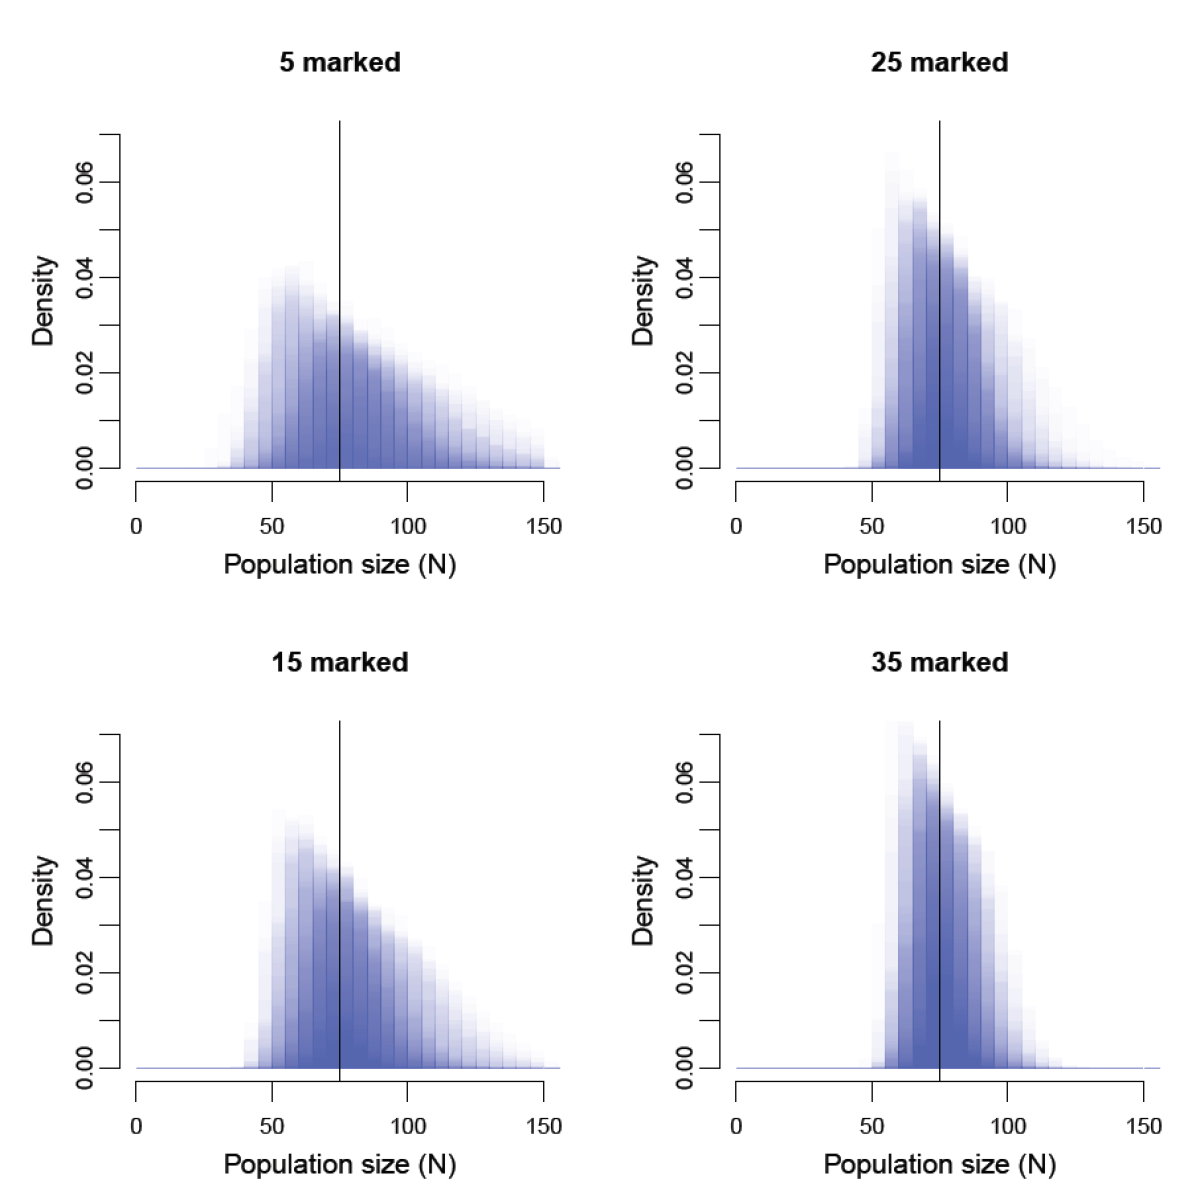
\includegraphics[width=4in,height=4in]{Ch19-PartialID/figs/Nposts2.png}
  \caption{Overlaid posterior distributions of $N$ from 100 simulations
    for four levels of marked individuals.}
  \label{partialID.fig.nposts}
\end{figure}

Without any marked individuals in the population, the posterior
distribution of $N$ turned out to be highly skewed, but the mode was
still an approximately (frequentist) unbiased point estimator of
$N$. As anticipated, posterior precision increased substantially with
the proportion of marked individuals (Table \ref{partialID.tab.sim} and
Fig. \ref{partialID.fig.nposts}). The relative root-mean squared
error decreased from 0.246 when no individuals were marked to 0.085
when 35 individuals were marked
(Table \ref{partialID.tab.sim}). Coverage was nominal for all values of
$m$ and posterior skew greatly diminished with increasing $m$ (Table \ref{partialID.tab.sim}).


\begin{table}[ht]
\centering
\caption{Posterior mean, mode, and associated relative RMSE for simulations in
  which $m$ of $N$=75 individuals were marked. One hundred simulations of each case were conducted. Table taken from \citet{chandler_royle:2012} }
\begin{tabular}{llrrrrr}
     \hline
     &	Parameter    &	Mean   &	rRMSE  & Mode   & rRMSE &	BCI    \\
     \hline
 m=0 &	$N$          &	85.866 &    0.259 & 77.720 &    0.242 & 0.950  \\
     &	$\lambda_0$  &	0.506  &	0.180 &	0.488  &	0.182 &	0.960  \\
     &	$\sigma$     &	0.495  &	0.115 &	0.486  &	0.113 &	0.960  \\
     \hline
 m=5 &	$N$          &	80.898 &    0.184 & 76.360 &    0.182 & 0.970  \\
     &	$\lambda_0$  &	0.510  &    0.178 & 0.494  &    0.180 & 0.950  \\
     &	$\sigma$     &	0.496  &    0.089 & 0.488  &    0.086 & 0.970  \\
     \hline
 m=15&	$N$          &	79.028 &    0.148 & 76.250 &    0.147 & 0.950  \\
     &	$\lambda_0$  &	0.508  &    0.163 & 0.494  &    0.164 & 0.950  \\
     &	$\sigma$     &	0.496  &    0.073 & 0.492  &    0.071 & 0.970  \\
     \hline
 m=25&	$N$          &	77.765 &    0.114 & 75.810 &    0.113 & 0.950  \\
     &	$\lambda_0$  &	0.511  &    0.153 & 0.498  &    0.157 & 0.950  \\
     &	$\sigma$     &	0.496  &    0.067 & 0.493  &    0.065 & 0.940  \\
     \hline
 m=35&	$N$          &	76.446 &    0.085 & 74.900 &    0.085 & 1.000  \\
     &	$\lambda_0$  &	0.513  &    0.142 & 0.501  &    0.144 & 0.950  \\
     &	$\sigma$     &	0.497  &    0.056 & 0.493  &    0.057 & 0.940  \\
 \hline
\end{tabular}
\label{partialID.tab.sim}
\end{table}

As we saw in the previous chapter, the spatial correlation in unmarked
counts can be sufficient to obtain estimates of movement and detection
parameters. However, only marked and thus identifiable individuals
provide us with direct information about these parameters and may well
dominate estimates.  To single out the contribution of marked and
unmarked individuals to parameter estimates, we re-ran the same
simulations but let $\sigma$ and $\lambda_0$ be updated based solely
on the data of marked individuals. Results are summarized in
Table \ref{partialID.tab.sim2}.  We see that if we update $\lambda_0$
and $\sigma$ based on marked individuals only, estimates of these
parameters are more biased and less precise. For estimates of $N$,
especially for $m$= 5 and $m$ = 15, we observe a stronger positive
bias, lower accuracy and considerably lower BCI coverage as compared
to when both marked and unmarked individuals contribute to parameter
estimates (Table \ref{partialID.tab.sim2}). Thus, unmarked individuals
do actually contribute noticeably to estimating model parameters.

\begin{table}[ht]
\centering
\caption{Posterior mean, mode, and associated relative RMSE for simulations in
  which $m$ of $N$=75 individuals were marked and unmarked individuals
  did not contribute to estimating $\lambda_0$ and $\sigma$.
  One hundred simulations of each case were conducted. }
\begin{tabular}{llrrrrr}
\hline
     &	Parameter    &	Mean   &	RMSE  &	Mode   &	RMSE &	BCI    \\
     \hline
 m=5 &	$N$          &	88.621 &	0.369 &	83.139 &	0.421 &	0.810  \\
     &	$\lambda_0$  &	1.255  &	1.247 &	0.606  &	1.148 &	0.950  \\
     &	$\sigma$     &	0.472  &	0.252 &	0.426  &	0.333 &	0.910  \\
     \hline
 m=15&	$N$          &	81.031 &	0.192 &	78.361 &	0.175 &	0.820  \\
     &	$\lambda_0$  &	0.535  &	0.281 &	0.476  &	0.284 &	0.970  \\
     &	$\sigma$     &	0.503  &	0.109 &	0.490  &	0.107 &	0.940  \\
     \hline
 m=25&	$N$          &	78.206 &	0.129 &	76.594 &	0.123 &	0.920  \\
     &	$\lambda_0$  &	0.531  &	0.204 &	0.496  &	0.202 &	0.960  \\
     &	$\sigma$     &	0.497  &	0.081 &	0.489  &	0.084 &	0.950  \\
     \hline
 m=35&	$N$          &	76.833 &	0.099 &	75.422 &	0.096 &	0.940  \\
     &	$\lambda_0$  &	0.528  &	0.192 &	0.505  &	0.186 &	0.940  \\
     &	$\sigma$     &	0.499  &	0.069 &	0.493  &	0.070 &	0.960  \\
 \hline
\end{tabular}
\label{partialID.tab.sim2}
\end{table}


\section{Incorporating telemetry data}
\label{partialID.sec.telemetry}

As we expected, parameter estimates of spatial mark-resight models get
better the more marked individuals we have in our study
population. While this is great advice in theory, it may not be very
helpful in practice, especially when dealing with animals that are
hard or somewhat dangerous to capture, such as large
carnivores. Oftentimes, studies involving the physical capture of such
animals will employ telemetry tags in order to learn about the study
species' spatial ecology and behavior. In the context of spatial
mark-resight models, the actual locations
collected by telemetry tags can provide detailed information on individual location and movement, and being able to incorporate this information directly into the SMR model should improve estimates of these parameters, especially when resighting information is sparse.

%% XXXXX Andy: seems like a cite to the JAPPLE paper would be good
%% around here?
% XX RS: We cite it in the last paragraph of this section. 

So how could we combine resighting data and telemetry data in a
unified mark-resight model? Recall that the basic SCR model underlying
all the SMR models we discuss here uses a Gaussian kernel to describe
the trap encounter model.  By using this function, we can relate the
parameters $\sigma$ and ${\bf s}_{i}$ directly to those from a
bivariate normal model of space usage, with mean = ${\bf s}_{i}$, and
variance-covariance matrix ${\bm \Sigma}$, where the variance in both
dimensions is $\sigma^2$ and the covariance is 0. Ordinarily, these
parameters are estimated directly from the spatial distribution of
individual captures/resightings. Telemetry data, however, provide more
detailed information on individual location and movement, since the
resolution and extent of the data are not limited by the trapping grid
and potentially more locations can be accumulated through telemetry
than resighting (depending on the monitoring frequency and resighting
rates of individuals).

By assuming that the $R_i$ locations of individual $i$, ${\bf l}_{i}$ (consisting of a pair of x and y coordinates, $l_{ix}$ and $l_{iy}$), are a bivariate normal (BVN) random variable:
\[
{\bf l}_i\sim {\mbox BVN} ({\bf s}_i,{\bm \Sigma})
\]
we can estimate $\sigma$ as well as ${\bf s}_{i}$ for the collared individuals directly from telemetry locations, using their full conditional distributions:
\[
[\sigma|{\bf l},{\bf s}] \propto \left\{\prod_{i=1}^m \prod_{r=1}^{R_{i}} \frac{1}{2 \pi \sigma^2} {\exp}\left(-1/2 \left[ \frac {(l_{irx}-s_{ix})^2} {\sigma^2} + \frac{(l_{iry}-s_{iy})^2}{\sigma^2} \right]\right)\right\}*[\sigma]
\]
and
\[
[{\bf s}_i|{\bf l},\sigma] \propto \left\{\prod_{r=1}^{R_{i}} \frac{1}{2 \pi \sigma^2} {\exp}\left(-1/2 \left[ \frac {(l_{irx}-s_{ix})^2} {\sigma^2} + \frac{(l_{iry}-s_{iy})^2}{\sigma^2} \right]\right)\right\}*[{\bf s}_{i}]
\]

For the unmarked individuals ${\bf s}_{i}$ are estimated as described
before conditional on their latent encounter histories.  Note that the
bivariate normal model assumes that locations are independent of each
other. If you have frequent telemetry fixes, for example from GPS
collars that report animal locations every few hours or more, this
assumption seems unrealistic and it might be advisable to thin your
telemetry data (maybe to daily fixes) in order to approximate
independence.  Alternatively, movement models could be used that
acknowledge the temporal correlation in location data. We suggested
some possible movement models in Chapt. \ref{chapt.search-encounter}.
Not all marked individuals need to be telemetry-tagged, but telemetry
data should correspond to the period over which resighting surveys
were conducted (as we discussed in Chapt. \ref{chapt.scr0}, both the
${\bf s}_i$ and $\sigma$ should only be interpreted against the
specific sampling period). Further, telemetry data need to be
independent of the resighting data.

Again, implementation of this model extension is straight-forward,
both in {\bf JAGS} and {\bf R}. Take the SMR model description for the
case where $m$ is known (Panel \ref{partialID.panel.knownm}). Then,
all we have to do is add a description of the bivariate normal model
for the telemetry locations, here {\tt locs}, into the loop over the
$m$ marked individuals: 
{\small
\begin{verbatim}
[...parts of model code omitted...]

for(i in 1:m) {

  sm[i,1] ~ dunif(xlim[1], xlim[2])
  sm[i,2] ~ dunif(ylim[1], ylim[2])

  #telemetry model
  for (r in off1[i]:off2[i]){
  locs[r,1]~dnorm(sm[i,1], 1/(sigma^2))
  locs[r,2]~dnorm(sm[i,2], 1/(sigma^2))
  }

  for(j in 1:J) {
    distm[i,j] <- sqrt((sm[i,1]-X[j,1])^2 + (sm[i,2]-X[j,2])^2)
    lambdam[i,j] <- lam0*exp(-distm[i,j]^2/(2*sigma^2))
    y[i,j]~dpois(lambdam[i,j]*K)
    }
  }

[...parts of model code omitted...]
\end{verbatim}
}
The data object {\tt locs} is a table with all $\sum_i^m R_i$
telemetry locations. The two vectors {\tt off1} and {\tt off2}
describe which subset of this matrix belongs to individual $i$. So if,
say, the locations for individual 1 are contained in the first 10 rows
of {\tt locs}, {\tt off1} and {\tt off2} would be 1 and 10 for $i=1$;
and if the locations of individual 2 are in the following 15 rows,{\tt
  off1} and {\tt off2} for $i=2$ would be 11 and 25, and so on. For
the implementation of this SMR model with telemetry data in {\bf R},
see the {\tt scrPID.tel} function in {\tt scrbook}. In a nutshell, in
the MCMC algirithm we replaced the Metropolis-Hastings updating steps
for $\sigma$ and activity centers, ${\bf s}_i$, of marked individuals, which were originally
conditional on the resighting data, with updating steps conditional on
the telemetry data. This is not quite what the above {\bf JAGS} code
does; rather {\bf JAGS} will update these parameters conditional on
both the telemetry \emph{and} the resighting data. We could easily
re-write {\tt scrPID.tel} to do that, but believe that for most
applications, the information on location and movement contained in
the telemetry data will outweigh that in the resighting data, so that
the resulting loss of information should be minimal.

\subsection{Raccoons on the Outer Banks of North Carolina}

\citet{sollmann_etal:2012ecol} applied a spatial mark-resigh model
with telemetry data to a camera-trap and radio-telemetry data set from
the raccoon population on South Core Banks, a barrier island within
Cape Lookout National Seashore, North Carolina. Between May and
September 2007, 131 raccoons were marked with dog collars and large
individually numbered cattle tags. Individuals were marked throughout
the island, so that (a) we do not have to deal with sensitivity to
choice of the state-space, because it is clearly defined by nature;
and (b) it is reasonable to assume that marked raccoons are a random
sample of individuals from this state-space.  Of the 131 tagged
individuals, 44 were also equipped with radio collars. Collared
individuals were located using a VHF receiver and antenna, and their
locations were estimated approximately weekly. Twenty camera traps
were set up along the length of South Core Banks and camera trapping
data collected between October 1 2007 to January 22 2008 constituted
the resighting data in this analysis. During this period 104 marked
individuals, 38 radio-collared, were alive and available for
resighting with camera traps.

\begin{figure}[ht]
  \centering
  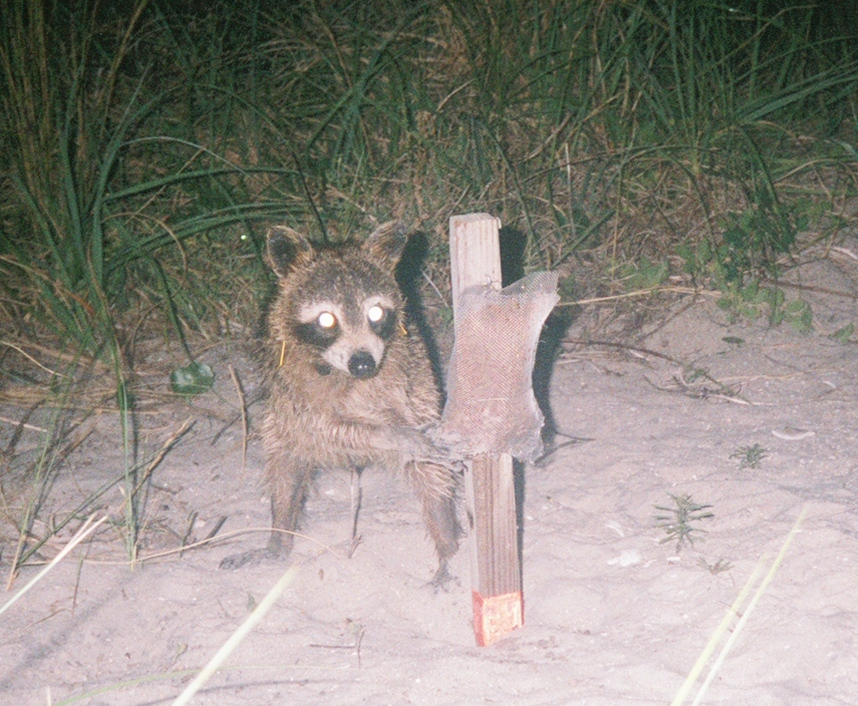
\includegraphics[width=4in]{Ch19-PartialID/figs/Raccoon_pic.png}
  \caption{Camera trap picture of a raccoon marked with a cattle tag that cannot be read to determine individual identity. Taken on South Core Banks, North Carolina.
({\it Photo credit: Arielle Parsons})}
  \label{partialID.fig.raccoon}
\end{figure}

The state-space ${\cal S}$ was the entire area of South Core Banks
island. A change in the number of photocaptures over the course of the
study suggested a variation of detection rate with time. Since date
recording in cameras malfunctioned, photographic records could only be
assigned to the time interval between subsequent trap checks, and
these intervals between checks are referred to as sampling
occasions. These occasions ranged from 2 to 43 days; $\lambda_0$ was
standardized to 7-day intervals and allowed to change with sampling
occasion. Since not all pictures of marked raccoons could be
identified to the individual level, the authors applied the correction
factor $c$ as described in Sec. \ref{partialID.sec.IDrate}, estimated
separately for each occasion.

Camera-traps recorded 117 pictures of unmarked raccoons, 33 pictures
of 18 marked and identifiable raccoons, and 49 records of marked but
not individually identifiable individuals
(Fig. \ref{partialID.fig.raccoon}). An average of 16.32 telemetry
locations (SD 4.91) were collected for each of the 38 collared
individuals. Raccoon abundance on the island was estimated at 186.71
(SE 14.81) individuals, which translated to a density of 8.29 (SE
0.66) individuals per km$^2$. Parameter estimates are listed in
Table \ref{partialID.tab.raccoons}.

\begin{table}%[hb]
\centering
\caption{Summary statistics of posterior distributions
from spatial mark-resigh model for raccoon camera trapping and telemetry data. Baseline trap encounter rate $\lambda_0$ was standardized to 7-day intervals; $\lambda_0$ and the probability of identifying a picture of a marked individual, $c$, were allowed to vary among the 6 sampling occasions (t); $\sigma$ is estimated from telemetry data of 38 radio-collared individuals.}
\begin{tabular}{lrrrrr}
\hline
   &	Mean (SE) &	2.5\% &	50\%	& 97.5\% \\
 \hline
$N$	& 186.71 (14.81) & 162 & 185	& 220 \\
$D$	& 8.29 (0.66)	& 7.19	& 8.22	& 9.77 \\
$\lambda_0$ (t=1)	& 0.24 (0.05) & 0.16 & 0.23 & 0.34 \\
$\lambda_0$ (t=2)	& 0.40 (0.08)	& 0.26	& 0.39	& 0.57 \\
$\lambda_0$ (t=3)	& 0.11 (0.03) & 0.06 & 0.11	& 0.17 \\
$\lambda_0$ (t=4)	& 0.30 (0.07)	& 0.17	& 0.29	& 0.46 \\
$\lambda_0$ (t=5)	& 0.03 (0.01)	& 0.02	& 0.03	& 0.06 \\
$\lambda_0$ (t=6)	& 0.03 (0.01)	& 0.02	& 0.03	& 0.05 \\
$\sigma$	& 0.49 (0.01)	& 0.47	& 0.49	& 0.51 \\
$c$ (t=1)	& 0.55 (0.09)	& 0.38	& 0.55	& 0.71 \\
$c$ (t=2)	& 0.39 (0.11)	& 0.18	& 0.39	& 0.62 \\
$c$ (t=3)	& 0.29 (0.11) & 0.11	& 0.29	& 0.52 \\
$c$ (t=4)	& 0.38 (0.16)	& 0.10	& 0.36	& 0.71 \\
$c$ (t=5)	& 0.38 (0.16)	& 0.10	& 0.36	& 0.71 \\
$c$ (t=6)	& 0.30 (0.14)	& 0.08	& 0.29	& 0.60 \\
 \hline
\end{tabular}
\label{partialID.tab.raccoons}
\end{table}

In this study, although a large number of raccoons were tagged,
photographic data of these tagged individuals were surprisingly
sparse. Analysis of the photographic data set without the telemetry
data did not render usable estimates as parallel Markov chains did not
converge. One reason for the relatively sparse data was the camera
trap study design: traps were spaced on average 1.77 km apart, which
is about 3.5 times $\sigma$. Consequently, very few individual
raccoons were photographed at more than one trap. Under these
circumstances, the telemetry data provide the necessary spatial
information to estimate $\sigma$ and the activity centers of
individual animals and thus make other model parameter
estimable. Similarly, in a camera-trapping study on Florida panthers
(\emph{Puma concolor coryi}), \citet{sollmann_etal:inprepjapplecol},
including telemetry data from the 3 individuals that were collared and
known to use the study area resulted in density estimates with
considerably higher precision as compared to preliminary estimates
\emph{without} telemetry location data, reducing the width of the 95
\% BCI by about 60 \%. Such improvements in precision of estimates is
especially important when we are interested in changes in the
population over time.


\section{Marked Animals Are Aot a Random Sample From the State-Space}

As discussed in Sec. \ref{partialID.sec.random}, all the previously
developed SMR models assume that marked individuals are a random
sample, both spatially and demographically, from the population of the
state-space. For many studies it may not be feasible to strive to meet
or approximate this assumption and it is thus important to generalize
SMR models to situations where marking does not take place throughout
${\cal S}$. If you think about it, even if you set up marking traps
throughout the state-space, individuals at the border of ${\cal S}$
would be exposed to fewer traps and be less likely to be caught, thus
creating a gradient in the proportion of marked to unmarked animals
(although if ${\cal S}$ is large enough this is probably negligible).
% XXXX RC: This last sentence doesn't seem to get at the key point,
% i.e. that the marked guys can almost never be assumed to be
% uniformly distributed in S.
%% Andy sez: but see my email from the morning of 3/24. Can you do a
%% random sample of traps and make a design-based argument here?
 Here, we will describe
%develop 
one tentative approach to dealing with this situation, by having marked individuals be a random (uniformly distributed) sample from a smaller region within ${\cal S}$, say ${\cal B}$.
The central point of this approach is that it establishes a spatial context for the marked part of the population. This spatial context is independent of ${\cal S}$ -- ${\cal B}$ remains constant -- and it provides a formal distribution of marked animals -- uniform in ${\cal B}$, none outside of ${\cal B}$ -- so that unmarked animals can be distributed in a way that overall density is constant.


\subsection{Marked animals are uniformly distributed in a smaller
  area}


%%% XXX Andy sez: not sure what to make of all of this.  By Richard's
%%% comments I gather that it is perhaps too experimental at this
%%% point. Can it be thinned down a bit to not say too much?

Imagine we perform an area search in a square, ${\cal B}$, for some species we want to study, maybe a reptile, and we mark all individuals we encounter. We conduct our sampling in a way that we can assume that the individuals we marked are uniformly distributed in ${\cal B}$. This also entails the assumption that ${\cal B}$ can be clearly defined. We will come back to these assumptions in a minute. We then perform resighting surveys of some sort in an area that overlaps ${\cal B}$, so that, when we set a state-space around our resighting locations, ${\cal B}$ is completely contained within ${\cal S}$ (Fig. \ref{partialID.fig.Box}), and we assume that the number of marked animals, $m$, is known. We further assume that individuals that were marked in ${\cal B}$ continue to live within ${\cal B}$ when resighting surveys are conducted, i.e. their activity centers do not shift during the complete mark-resight study. That means that we assume population closure across both the marking and the resighting part of the study.
% XXXX RC: This also assumes that there are no marked activity centers outside of B, which I think will be impossible and should be mentioned... again.

Let the total population of ${\cal B}$ be $N_B$. % XXXX Suggest: $N({\cal B})$?
% XXXX After defining N(B), I would establish that, under the
% assumption that of uniform *marginal* density, the expected values
% for each N are as follows (when using data augmentation):
% E[N] = M*psi
% E[N marked guys in B] = M*psi*theta
% E[N unmarked guys in B] = M*psi*(1-theta)
% E[N unmarked gusy outside of B] = M*psi*pi, where pi is (A(S)-A(B))/A(S)
Under the conditions specified above, the number of marked animals $m$ can be described as the outcome of a binomial random variable
\[
m \sim \mbox{Binomial}(\theta, N_B)
\]
where $\theta$ is the probability that an animal living in ${\cal B}$ is marked. Remember that, by definition, all marked animals live inside ${\cal B}$. We now have to make sure that unmarked individuals get distributed across ${\cal S}$ and ${\cal B}$ so that \emph{overall} density is constant. % XXXX RC: I think this should be stated as a (possibly) reasonable assumption, instead of something that "we have to make sure" is true
Let ${\cal A}$ be ${\cal S} - {\cal B}$, % XXXX RC: instead of a "minus" sign, I think you want $S \ni B$ or whatever the appropriate geometric symbol is.
i.e., the area of ${\cal S}$ \emph{not} covered by ${\cal B}$ (Fig. \ref{partialID.fig.Box}). Then, the proportion of $N$ that should fall inside ${\cal B}$, say $\pi_B$, can be expressed as ${\cal B}/({\cal A}+{\cal B})$. Consequently, the proportion of $N$ in ${\cal A}$, $\pi_A$,
% XXXX RC: You need to distinguish between S and the area of S, which could be denoted A(S) or something.
is ${\cal A}/({\cal A}+{\cal B})$.
Conditioning $\pi_B$ on being an unmarked animal, % XXXX RC: rephrase
we obtain
\[
 \pi_B | unmarked = \frac{(1-\theta)* \pi_B}{U/N}
\]
And we can use this conditional probability as prior probability for the activity centers of unmarked individuals to fall within {\cal B}.
In other words, we now have two sets of priors for activity centers.
% XXXX RC: I don't think this is the prior for activity centers. Under
% this model, all the activity centers have a uniform prior, but
% density is different for the 3 groups. That is why I would focus on
% the expected values of N that I listed above.
For marked animals, $[s_i]\sim \mbox{Uniform}({\cal B})$. For unmarked animals, we introduce a binary variable, say $b$, and let $b=1$ mean that $s_i$ lies within ${\cal B}$; then $[s_i]\sim \mbox{Bernoulli}(pi_B|unmarked)$.
Because manipulating areas that are not simple rectangles (in this example, ${\cal A}$) in {\bf JAGS} is not straight forward, we wrote our own MCMC algorithm for this model, which can be found in the {\tt scrbook} package by invoking {\tt scrPIDBox}. A full example of how to simulate and analyze data under this model is given on the help page for {\tt scrPIDBox}.

\begin{figure}[ht]
\begin{center}
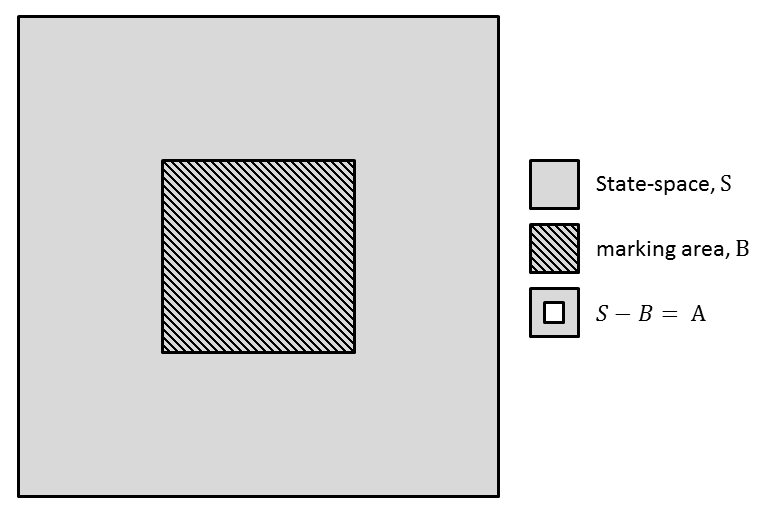
\includegraphics[width=5in]{Ch19-PartialID/figs/scrPIDBox.png}
\end{center}
\caption{
Relationship between marking area ${\cal B}$ and state-space, ${\cal S}$.
}
\label{partialID.fig.Box}
\end{figure}

The above %described
model is an approach to specifying a spatial reference frame for
marked individuals if these are not sampled uniformly from ${\cal S}$,
and provides us with the ability to distribute unmarked individuals
% XXXX RC: This reads as though "we" are distributing unmarked
% individuals around in space. I think it should say that this is a
% model that is reasonable if overall density can be assumed to be
% constant and the activity centeres of the marked guys are all
% uniformly distriubted within B.
proportionally between the marking area and the rest of the state-space, so that an overall uniform density is obtained. Some of the assumptions of the model, however, are reminiscent of traditional capture-recapture and thus, suffer from the same shortcomings. ${\cal B}$ needs to be clearly defined as the area the marked individuals live in, but how do we define it? Imagine again that ${\cal B}$ is a quadrad search plot. Surely, we could capture an individual at the edge of the plot, whose activity center is located \emph{off} that plot. Not accounting for this effect would overestimate density in ${\cal B}$. This is the equivalent of  having to define an effective area sampled in traditional capture-recapture in order to estimate density. Further, we assume that $\theta$, the probability of an individual within the plot being marked is the same for all individuals in ${\cal B}$. But we discussed early on in this book that this is unlikely to be true, because exposure to sampling depends on an individual's home range overlap with the sampled area. So individuals near the edge of ${\cal B}$ are less likely to be marked than those in the center, assuming we dispense marking effort uniformly across ${\cal B}$ (maybe we could counteract this effect to some extent by creating a decreasing gradient of sampling effort from the edge of the plot to the center).

\subsection{Combining marking and resighting models}

% XXXX I would remove this section, and instead focus on the solution
% that we know works: develop a model for spatial variation in the
% density of marked guys. We know this works because you imagine
% ignoring all of the unmarked guys and just estimating the abundance/density of
% marked guys. In that case, the only thing that differs from a
% standard SCR model is that we need to use an inhomogeneous point
% process because the marked guys will not be uniformly distributed in
% S. Istead, their density will almost surely decrease with distance
% from the traps where they were marked. There are several different
% ways of modeling this decrease in density. Once that is done, the
% IPP for the unmarked guys can be modeled by assuming that overall
% density is constant. Even if it isn't, you could theoretically
% develop any IPP for the unmarked guys too.

We can look at this approach from a slightly different
angle. Effectively, what we did here is combine a non-spatial capture
recapture model -- more specifically, model $M_0$ with equal capture
probability -- for the marking process with a spatial mark-resight
model for the resighting process. In our simplified example, we only
have a single marking occasion, but we can estimate $\theta$, the
probability of being captured and marked, because we have enough
information about how many unmarked individuals occur in ${\cal B}$
coming from the spatial resighting model. While the underlying
assumptions of the non-spatial marking model are questionable, we
believe that the idea of combining marking and resighting into a
unified model holds the key to developing a generalized spatial
mark-resight model that does not rely on animals being marked
throughout ${\cal S}$, at least when marking and resighting occur in a
short enough time frame that the population can be assumed closed. As
such, in spite of some shortcomings, the present approach is an
important conceptual step forward. We can think of alternative
distributions for marked individuals to move away from a completely
non-spatial description of the marking process; for example, activity
centers of marked individuals could follow a bivariate normal
distribution around the centroid of the marking array or plot, so that
the probability of being a marked individual is conditional on where
you live and decreases with distance to the collection of marking
locations. This avoids having to arbitrarily define an area, ${\cal
  B}$, but is still a simplification of the actual marking process. We
have not yet implemented this approach.  The essence of all of this is
that including the marking process into an SMR model provides a
spatial context for marked individuals, so that the resighting part of
the model is no longer sensitive to the choice of the state-space. The
next steps will be to develop a fully spatial model, where both the
marking and the resighting process are spatially explicit, and to
extend these models to the situation we can no longer use the
information from the marking process directly to provide spatial
context for marked individuals, because too much time passed between
marking individuals and resighting them, so that the assumption that
activity centers remain stationary is no longer reasonable.


%\subsection{Marked animals follow a bivariate normal distribution around the centroid of the marking array}
% In this approach we assume that marking of animals takes place across some area and that in the time between marking and resighting, the marked animals, the number of which is unknown, distribute themselves according to a bivariate normal distribution centered on the centroid of the marking area or grid, say $C_m$. This could happen in two fashions: (a) animals spread out around the marking area, but most stay close while only few venture out further; or (b) this represents the original distribution of marked animals, because animals living in the center of the markign grid have a higher probability to be marked than those living on the edges, so that the density of marks is higher near the centriod of the marking grid and decreases (here, following a bivariate normal distribution) as we move a away from that centroid.
% This model allows us to describe the probability of an animal being marked as a function of the distance of its activity center to $C_m$




\section{Summary and Outlook}

In this chapter we combined SCR models and the spatial model for
unmarked populations to derive a spatial mark-resight model, which
accomodates that part of the population is individually identifiable,
usually through artificial tags. Under the assumption that marked
individuals are a random sample, both demographically and spatially,
from the state-space, the basic model with known number of marked
individuals and 100\% individual identification of marked is easily
modified for situations where the number of marked individuals is
unknown, or where marked animals can sometimes not be identified to
individual level. As expected, having marked individuals in the study
population improved accuracy and precision of parameter estimates when
compared to fully unmarked populations, but we also saw that the
spatial counts of unmarked individuals still contribute information to
parameter estimates. Finally, we present an approach of how to
incorporate telemetry location data into the spatial mark-resight
model to inform estimates of $\sigma$ and activity centers. Just as in
SCR, the spatial mark-resight models can account for a variety of
factors that may influence individual movement and detection, as well
as survey-related parameters, and we saw one example for the Canada
geese, where $\sigma$ was sex-specific.

Many details of SMR models remain to be explored. We mentioned the
assignment of marked but unidentified records to actual marked
individuals based on their spatial location, which provides some
(though imperfect) information of their identity
(Sec. \ref{partialID.sec.IDrate}). Similarly, records where the marked
status cannot be determined could potentially be included in the model
as some form of overall correction factor on detection. GPS telemetry
devices and their ability to collect location data with much higher
frequency offer the opportunity to assign records of collared animals
to individuals based on how close to a given camera the collared
individuals were, both in space and time. In this scenario, individual
identity itself could be expressed probabilistically, leading to an
SMR model accounting for potential misidentification. All these
possible extensions can tailor SMR models to specific survey
techniques.

A fundamental assumption of all the SMR models developed in this chapter was that marked animals are a
random sample from ${\cal
  S}$. This simplifies the model as we can assume a homogeneous point process for both the marekd and the unmarked part of the population. While this is a convenient situation, it is neither likely to arise often in real life, nor a necessary assumption.  
If marked animals are not a random sample from
${\cal S}$, we need to describe their distribution in the state-space using an adequate point-process that will almost always be inhomogeneous across ${\cal S}$. 
We mention two possible approach -- a uniform (homogeneous) point process over a smaller area within ${\cal S}$, and a bivariate normal distribution around the centroid of the marking locations, so that density of marked animals decreases with distance to that centroid. 

Both formulations effectively attempt to describe the distribution of marks in space as a consequence of the spatial nature of the marking process. We believe that another way to approach this problem is to combine spatially explicit models for the marking process and the resighting process. Where  marked animals were captured carries information on their spatial distribution, and it should be possible to make use of this information by formulating an integrated spatial capture-mark-resighting model. Such approaches have been developed in a non-spatial CR framework \citep{matechou_etal:2013, pledger_etal:2009}, but to our knowledge have not yet been addressed in the context of SCR.

 Spatial mark-resight models are a fairly
new development and work on how to relax the spatial component of the
random sample assumption and formulate adequate point-process models for the distribution of marks is ongoing. While there is still a lot of work to be done, we believe that SMR modeling holds the
potential to address a wide range of population estimation problems
when dealing with animals that cannot be identified based on natural
marks.



% \subsection{Sensitivity to the state-space}

% While the formulation of spatial mark-resight models for a known
% number of marked indivduals, $m$, is straight forward, these model
% have one major caveat: because we fix the size of the marked part of
% our population, total population size $N$ no longer scales with the
% area of the state-space. While the number of unmarked individuals can
% go up as ${\cal S}$ increases in size, $m$ is fixed by design. If our
% data contain all-zero encounter histories for some of the marked
% individuals, we have no immediate information about where in the
% state-space these never observed individuals live (apart from the
% vague information that they probably do not live in the middle of the
% trap array). As we increase ${\cal S}$, the area over which these marked
% unobserved individuals can live increases, too -- and consequently,
% their density decreases.  As a result, we find that density estimates
% from spatial mark-resight models with a known number of marks are
% sensitive to choice of the state-space -- as we increase ${\cal S}$,
% density estimates go down.  This is, of course, a highly undesirable
% quality in a density model. {\bf XXXXX Not a property of the model,
%   but rather of misspecifying something! We need to figure this
%   out.... XXXXXX}
% While this is an area of active research,
% we believe that under certain circumstances, the problem of
% sensitivity to the state-space can be avoided: If all marked animals
% are resighted at least once, we have some information about where in
% the state-space they live -- their activity centers must be close
% enough to the trap array for them to be resighted on it. Thus, even if
% we increase the overall state-space, the possible locations for the
% activity centers of the marked individuals remain limited. The effect
% is that, irrespective of the state-space, the marked individuals refer
% to a constant area, instead of getting `diluted'. Even if marked
% individuals are not resighted, we might have other sources of
% information on where they resided during our study, such as telemetry
% locations. Again, this information gives us the ability to fix the
% area the marked individuals refer to irrespective of the size of ${\cal
%   S}$, avoiding bias in density estimates. For an example of how to
% include telemetry data into spatial mark-resight models, see
% Sec. \ref{partialID.sec.telemetry}. A third option that we have not
% formally explored ourselves is to explicitly include capture locations
% of marked individuals into the model. Once again, this would provide
% some spatial reference for the location of marked individuals within
% the state-space. Lastly, there are circumstances under which we know
% the exact state-space in which individuals were marked and are being
% resighted. For example, if we study the population of some species on
% an island, and the entire island's population is potentially exposed
% to marking efforts (see the raccoon example in
% Sec. \ref{partialID.sec.telemetry}). In this case there is no
% arbitrariness in choosing ${\cal S}$ -- it is the island. If none of
% these avenues is an option, there is always the possibility of
% treating the number of marked individuals as unknown (see
% Sec. \ref{partialID.sec.unknown}), which might be more realistic under
% most field situations anyway. You should not that while we discussed
% the problem of underestimating density with an increase in
% state-space, there is also the opposite risk: if we choose ${\cal S}$
% too small so that it does not contain the activity centers of all of
% the marked individuals, but we assume, by fixing $m$, that they are
% all part of the population, we will overestimate density -- just as we
% would if we chose ${\cal S}$ too small in a regular SCR setting. All
% this just emphaizes what we already stated in Chapt. \ref{chapt.scr0}:
% the state-space is an integral part of your spatial capture-recapture
% (or mark-resight) model and some thought should go into specifying it
% adequately.

% \subsection{MCMC for a spatial mark-resight model}

% Implementing a spatial mark-resight model in {\bf JAGS} is not
% trivial, % XXXX See the "scratch" directory and the .jag files for
%          % some examples of working around this issue in JAGS
% since the program does not accept partially observed
% multivariate nodes (in this case the partially observed individual
% encounter histories which we model as coming from a multinomial
% distribution). Therefore, knowing how to write your own MCMC algorithm
% comes
% in
% handy. You will find that we only have to make relatively
% simple modifications to the MCMC code we developed for regular SCR models in
% Chapt. \ref{chapt.mcmc}.
% Essentially, since we observe individual detections for the marked part of the population, we have to update only the unobserved part of ${\bf Y}$, and
% modify the updating steps for $z_i$ and $\psi$, the parameters introduced by data augmentation, to reflect some
% contribution to our
% knowledge of these parameters from the $m$ marked individuals.

% First, we set up an array to hold ${\bf Y}$, fill the first $m$ rows
% of the array with the $m$ observed individual encounter histories,
% then update ${\bf Y}$ for the unknown individuals only (note that the
% code is set up so that $n_{jk}$ contains both pictures of marked {\bf
%   and} unmarked individuals at $j$ and $k$):


% {\small
% \begin{verbatim}
% # set up placeholders and create vectors for marked and unmarked
%  Y <- array(NA, c(M, J, K))
%     nMarked <- nrow(y)
%     marked <- rep(FALSE, M)
%         marked[1:nMarked] <- TRUE
%         Y[1:nMarked, , ] <- y
%     z[marked] <- 1
%     Ydata <- !is.na(Y)
%     for (j in 1:J) {
%         for (k in 1:K) {
%             if (y[j, k] == 0) {
%                 Y[, j, k] <- 0
%                 next
%             }
%             unmarked <- !Ydata[, j, k]
%             nUnknown <- n[j, k] - sum(Y[!unmarked, j,k])
%             if (nUnknown < 0)
%                 browser()
%             probs <- lam[, j] * z
%             probs <- probs[unmarked]
%             probs <- probs/sum(probs)
%             Y[unmarked, j, k] <- rmultinom(1, nUnknown, probs)
%         }
%     }
% \end{verbatim}
% }

% When we know the number of marked individuals in the population estimating $N$ is reduced to etimating $U$. Thus, we only need to estimate the $z_i$ for $M-m$ unknown individuals and the updater for $z_i$ becomes:
% {\small
% \begin{verbatim}
% zUps <- 0
% seen <- apply(Y > 0, 1, any)
%    for (i in 1:M) {
%        if (seen[i] | marked[i])
%                 next
%        zcand <- ifelse(z[i] == 0, 1, 0)
%        ll <- sum(dpois(Y[i, , ], lam[i, ] * z[i], log = TRUE))
%        llcand <- sum(dpois(Y[i, , ], lam[i, ] * zcand,
%                   log = TRUE))
%        prior <- dbinom(z[i], 1, psi, log = TRUE)
%        prior.cand <- dbinom(zcand, 1, psi, log = TRUE)
%           if (runif(1) < exp((llcand + prior.cand) - (ll +
%                 prior))) {
%           z[i] <- zcand
%           zUps <- zUps + 1
%             }
%         }
% \end{verbatim}
% }
% Observe that while we skip the update of $z_i$ for the ``seen'' individuals (where  {\tt seen=TRUE} for any individual observed at least once and {\tt seen=FALSE} otherwise), {\tt seen} is defined based on ${\bf Y}$ and ${\bf Y}$ is updated at each iteration, so the $z_i$ for the observed but unmarked individuals are still updated.

% Finally, our update for $\psi$ needs to reflect that we are effectively only estimating $U$. In the full conditional beta distribution we have to replace $M$ with $M-m$ and $\sum z$ with $\sum z -m$:
% {\small
% \begin{verbatim}
%   psi<-rbeta(1,1+sum(w[!marked]),1+sum(!marked)-sum(w[!marked]))
% \end{verbatim}
% }
% The remainder of the code is essentially identical to the MCMC code for regular SCR models we developed in Chapt. \ref{chapt.mcmc}.
% You can find the full MCMC code (including the modeling options we'll discuss in the following sections) in the accompanying {\bf R} package {\tt scrbook} by invoking {\tt scrPID}.

% \subsection{Binomial encounter model}
% So far, we have only worked with Poisson encounter models for
% partially identifiable or unmarked populations. When we use a
% Bernoulli model instead, we have to make some changes to how we update
% the latent $y_{ijk}$, to ensure that a hypothetical individual
% receives at most a single observation at a given trap and occasion
% from the pool of $n_{jk}$ pictures. Thus, we move from a multinomial
% model
% where the same individual could be drawn repeatedly, to a sampling
% without replacement model(an individual drawn once at $j$ and $k$
% cannot be drawn again). The resuting full conditional distribution of
% the latent encounter histories is called a multivariate hypergemetric
% distibution; here is how we implement this in our MCMC algorithm:

% {\small
% \begin{verbatim}
%  Y <- array(NA, c(M, J, K))
% #[...]
%     for (j in 1:J) {
%         for (k in 1:K) {
%             if (y[j, k] == 0) {
%                 Y[, j, k] <- 0
%                 next
%             }
%             unmarked <- !Ydata[, j, k]
%             nUnknown <- n[j, k] - sum(Y[!unmarked, j,k])
%             if (nUnknown < 0)
%                 browser()
%             probs <- lam[, j] * z
%             probs <- probs[unmarked]
%             probs <- probs/sum(probs)
%             Y[unmarked, j, k] <- 0
%             guys <- sample(which(unmarked), nUnknown, prob = probs)
%             Y[guys, j, k] <- 1
%         }
%     }
% \end{verbatim}
% }


% {\bf R} makes it easy to implement the update of $\sigma$ and ${\bf
%   s}_i$ based on telemetry data and the above described full
% conditionals within our existing MCMC algorithm. We replace the
% current updating step for $\sigma$ with:
% {\small
% \begin{verbatim}
% #ntot = number of telemetry-tagged individuals
% #locs = list of length ntot; each element is a matrix
% #with telemetry locations
% #telID = vector with identifier for telemetry-tagged
% #individuals

% sigma.cand <- rnorm(1, sigma, delta[1])
% if (sigma.cand > 0) {

% llsig<-llsig.cand<-rep(NA, ntot)

% for (x in 1:ntot) {
% lls[x]<-sum(dmvnorm(x=locs[[x]],mean=c(S[telID[x],1],S[telID[x],2]),
% 			sigma=cbind(c(sigma^2,0), c(0,sigma^2)), log=T))
% lls.cand[x]<-sum(dmvnorm(x=locs[[x]],mean=c(S[telID[x],1],S[telID[x],2]),
% 	sigma=cbind(c(sigma.cand^2,0), c(0,sigma.cand^2)), log=T))
% 	}
%    if(runif(1) < exp( sum(lls.cand)  - sum(lls) ) ){
%     sigma<-sigma.cand
%     lam <- lam0*exp(-(D*D)/(2*sigma.cand*sigma.cand))
% 					}
% 			}
% \end{verbatim}
% }
% For the ${\bf s}_i$ we use an analogous updater for the
% telemetry-tagged individuals and the regular updater for individuals
% without associated telemetry location information.
% A full example can
% be found in the {\bf R} package {\tt scrbook}, by calling {\tt
%   scrPID.tel}.



% Further, if our data contain all-zero encounter histories
% for some of the marked individuals, we have no immediate information
% about where in the state-space these never observed individuals live
% (apart from the vague information that they probably do not live in
% the middle of the trap array). As we increase ${\cal S}$, the area
% over which these marked unobserved individuals can live increases, too
% -- and consequently, their density decreases. Even if we do not know
% $m$, we usually know an upper bound for it -- the total number ever
% caught before resighting. This upper bound does not change, no matter
% the size of the state-space, so again, at some point, estimates of $m$
% will hit the upper limit and after that, density will decrease as we
% increase ${\cal S}$. There is also the opposite risk: if we choose
% ${\cal S}$ too small so that it does not contain the activity centers
% of all of the marked individuals, but we assume, by fixing $m$, that
% they are all part of the population, we will overestimate density --
% just as we would if we chose ${\cal S}$ too small in a regular SCR
% setting. But this problem can be avoided much more easily, by
% increasing ${\cal S}$.






\bibliography{AndyRefs_alphabetized}

\end{document}